\begin{center}
	ĐỀ ÔN TẬP KIỂM TRA GIỮA HỌC KỲ I – MÔN VẬT LÝ 11\\
	Thời gian làm bài: 50 phút \\
	(Không kể thời gian phát đề)\\
\end{center}
\begin{enumerate}[label=\bfseries Câu \arabic*]
	\item \textbf{\textit{(1,5 điểm)}:}\\ Em đang đứng ở cuối tấm ván nhảy hồ bơi và bắt đầu nhún lên ván để nó dao động. Em sẽ nhận thấy rằng khi thay đổi tần số dao động đến một giá trị xác định $f$ nào đó thì tấm ván dao động với biên độ cực đại. 
	\begin{center}
		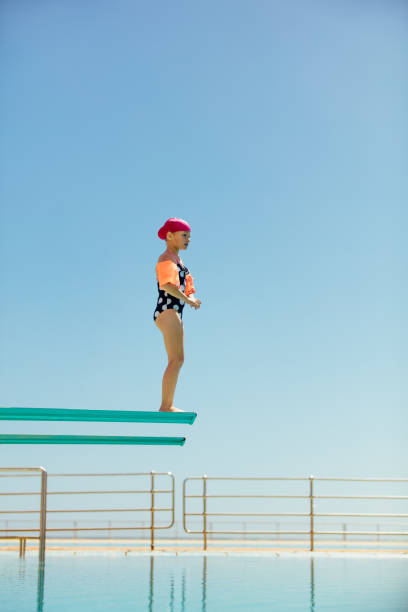
\includegraphics[width=0.25\linewidth]{../figs/D11-4-4}
		\captionof{figure}{Minh hoạ người nhún lên ván để ván dao động.}
	\end{center}
	\begin{enumerate}[label=\alph*)]
		\item Kết quả mô tả ở đề bài liên quan đến hiện tượng vật lý nào mà em đã được học? Điều kiện để xảy ra hiện tượng trên là gì?
		\item Nếu em di chuyển đến giữa tấm ván và lặp lại thí nghiệm như trên thì tần số $f$ sẽ cần phải lớn hơn, nhỏ hơn, hay bằng tần số ban đầu để ván dao động với biên độ cực đại? Em hãy đưa ra giải thích để chứng minh cho câu trả lời của em.
	\end{enumerate}
\hideall{
\begin{enumerate}[label=\alph*)]
	\item Khi người nhún lên tấm ván, người này đã tác dụng ngoại lực tuần hoàn lên ván làm ván dao động cưỡng bức. Khi thay đổi tần số của ngoại lực cưỡng bức đến giá trị bằng tần số dao động riêng của ván thì ván sẽ dao động với biên độ cực đại, đây là hiện tượng cộng hưởng.\\
	Điều kiện xảy ra hiện tượng cộng hưởng là tần số của ngoại lực cưỡng bức tác dụng lên hệ dao động bằng với tần số dao động riêng của hệ.
	\item Khi người nhún lên ván, tấm ván biến dạng đàn hồi và bắt đầu dao động. Ta có thể xem tấm ván như một lò xo có độ cứng $k$. Tần số dao động riêng của hệ ván và người
	$$f=\dfrac{1}{2\pi}\sqrt{\dfrac{k}{m}}$$
	với $m$ là khối lượng của người và ván.\\
	Nhận thấy rằng với cùng trọng lượng của người tác dụng lên ván, khi càng tiến vào gần đầu ván thì độ biến dạng của ván càng giảm, điều đó chứng tỏ rằng độ cứng của ván càng tăng $\left(k=\dfrac{P}{\Delta\ell}\right)$. Do đó, tần số dao động riêng của ván càng tăng khi người này tiến về đầu ván.\\
	Vậy khi người này tiến về phần giữa của ván thì $f$ phải lớn hơn giá trị ban đầu (khi đứng ở cuối ván) để ván dao động với biên độ cực đại.
\end{enumerate}
}
	\item \textbf{\textit{(2,5 điểm)}:}\\
	{Đồ thị li độ - thời gian của một vật dao động điều hoà được thể hiện như hình \ref{fig:4.1}. Dựa vào đồ thị, em hãy xác định
	\begin{center}
		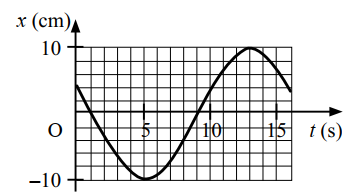
\includegraphics[width=0.45\linewidth]{../figs/D11-4-2}
		\captionof{figure}{Đồ thị li độ - thời gian của vật dao động điều hoà.}
		\label{fig:4.1}
	\end{center}
\begin{enumerate}[label=\alph*)]
	\item Biên độ dao động.
	\item Chu kì dao động.
	\item Tần số góc dao động.
	\item Tốc độ trung bình của vật trong thời gian $\SI{8}{\second}$.
	\item Vận tốc của vật tại thời điểm $t=\SI{12}{\second}$.
\end{enumerate}}
\hideall{
\begin{enumerate}[label=\alph*)]
	\item Biên độ dao động của vật $A=\SI{10}{\centi\meter}$.
	\item Chu kì dao động của vật: $T=\SI{16}{\second}$.
	\item Tần số góc dao động:
	$$\omega=\dfrac{2\pi}{T}=\xsi{\dfrac{\pi}{8}}{\radian/\second}$$
	\item Trong khoảng thời gian $\Delta t=\SI{8}{\second}=\dfrac{T}{2}$ vật đi được quãng đường $s=2A=\SI{20}{\centi\meter}$.\\
	Tốc độ trung bình của vật trong khoảng thời gian này
	$$v_\text{tb}=\dfrac{s}{\Delta t}=\dfrac{\SI{20}{\centi\meter}}{\SI{8}{\second}}=\SI{2.5}{\centi\meter/\second}.$$
	\item Tại thời điểm $t=\SI{5}{\second}$ vật qua vị trí $x=-A$, pha dao động của vật lúc này
	$$\varphi=\omega t+\varphi_0=\xsi{\pi}{\radian}\Rightarrow \varphi_0=\varphi-\omega t=\xsi{\pi}{\radian} -\left(\xsi{\dfrac{\pi}{8}}{\radian/\second}\right)\cdot\left(\SI{5}{\second}\right)=\xsi{\dfrac{3\pi}{8}}{\radian}$$
	Phương trình dao động của vật:
	$$x=A\cos\left(\omega t+\varphi_0\right)=\xsi{10\cos\left(\dfrac{\pi}{8}t+\dfrac{3\pi}{8}\right)}{\centi\meter}$$
	Phương trình vận tốc của vật:
	$$v=-\omega A\sin\left(\omega t+\varphi_0\right)=\xsi{-1,25\pi\sin\left(\dfrac{\pi}{8}t+\dfrac{3\pi}{8}\right)}{\centi\meter/\second}$$
	Tại thời điểm $t=\SI{12}{\second}$ thì vận tốc của vật có giá trị:
	$$v=-1,25\pi\sin\left(\dfrac{\pi}{8}\cdot12+\dfrac{3\pi}{8}\right)\approx\SI{1.5}{\centi\meter/\second}.$$
\end{enumerate}
}
\item \textbf{\textit{(3,0 điểm)}:}\\ {Một xe chạy trên đệm khí được mắc vào lò xo nhẹ có một đầu cố định như hình \ref{fig:4.2}. Khối lượng của xe là $\SI{0.12}{\kilogram}$ và xe dao động với biên độ $\SI{0.075}{\meter}$. Khi qua vị trí cân bằng, xe có tốc độ $\SI{0.524}{\meter/\second}$. Hãy xác định
\begin{center}
	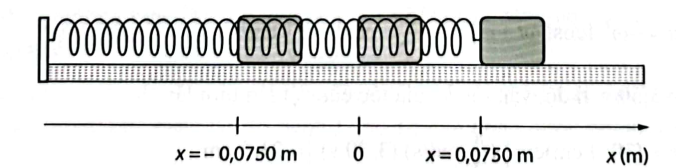
\includegraphics[width=0.7\linewidth]{../figs/D11-4-3}
	\captionof{figure}{Minh hoạ xe chạy trên đệm không khí.}
	\label{fig:4.2}
\end{center}
\begin{enumerate}[label=\alph*)]
	\item Độ cứng của lò xo.
	\item Gia tốc của xe khi nó ở vị trí biên dương.
	\item Cơ năng dao động của xe.
	\item Các vị trí xe có động năng gấp đôi thế năng.
\end{enumerate}}
\hideall{
	\begin{enumerate}[label=\alph*)]
		\item Khi xe qua VTCB, tốc độ của nó đạt cực đại:
		$$v_\text{max}=\omega A\Rightarrow \omega=\dfrac{v_\text{max}}{A}=\dfrac{\SI{0.524}{\meter/\second}}{\SI{0.075}{\meter}}\approx\SI{6.99}{\radian/\second}$$
		Độ cứng của lò xo:
		$$k=m\omega^2=\left(\SI{0.12}{\kilogram}\right)\cdot\left(\SI{6.99}{\radian/\second}\right)^2=\SI{5.86}{\newton/\meter}.$$
		\item Khi xe ở vị trí biên dương, gia tốc của xe:
		$$a=-\omega^2A=-\left(\SI{6.99}{\radian/\second}\right)^2\cdot\left(\SI{0.075}{\meter}\right)=\SI{-3.66}{\meter/\second^2}.$$
		\item Cơ năng của xe:
		$$W=W_\text{đ max}=\dfrac{1}{2}mv^2_\text{max}=\dfrac{1}{2}\cdot\left(\SI{0.12}{\kilogram}\right)\cdot\left(\SI{0.524}{\meter/\second}\right)^2=\SI{0.0165}{\joule}.$$
		\item Khi vật qua vị trí có động năng gấp đôi thế năng $W_\text{đ}=2W_\text{t}$ thì 
		$$W_\text{t}=\dfrac{1}{3}W\Leftrightarrow \dfrac{1}{2}kx^2=\dfrac{1}{3}\cdot\dfrac{1}{2}kA^2$$
		$$\Rightarrow x=\pm\dfrac{A}{\sqrt{3}}\approx\pm\SI{0.0433}{\meter}.$$
	\end{enumerate}
}
\item \textbf{\textit{(3,0 điểm)}:}\\ Một con lắc đơn gồm vật nhỏ khối lượng $\SI{50}{\gram}$ treo vào sợi dây có chiều dài $\SI{2.23}{\meter}$ tại nơi có gia tốc trọng trường $g$. Đồ thị vận tốc - thời gian của vật nhỏ khi con lắc dao động như ở hình \ref{fig:4.3}. Xác định
\begin{center}
	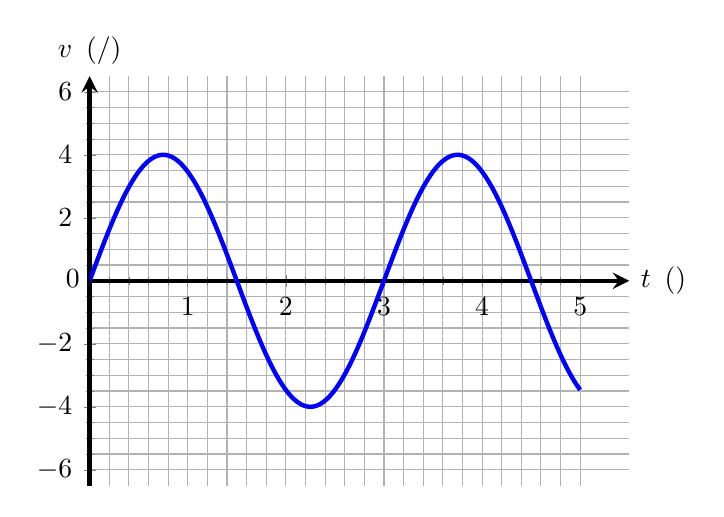
\begin{tikzpicture}  
		\begin{axis}[  ultra thick,
			xmin=0,  
			xmax=5.5,  
			xtick={0,1,...,5},
			ytick={-6,-4,...,6},
			minor x tick num=4,
			minor y tick num=3,
			ymin=-6.5,  
			ymax=6.5, 
			y=0.4cm,
			samples=300,
			axis lines=center, 
			grid style={step=1, color=gray!60!white},
			grid=both,
			xlabel=$t\ \left(\si{\second}\right)$, 
			ylabel=$v\ \left(\si{\centi\meter/\second}\right)$, 
			every axis y label/.style={at=(current axis.above origin),anchor=south},  
			every axis x label/.style={at=(current axis.right of origin),anchor=west},  ]
			\addplot [ultra thick, blue, smooth, domain=0:5] {4*cos(deg(2*pi*x/3-pi/2))}; 
		\end{axis}  
		\node[label={[left]90:0}] at (0,2.5){};
	\end{tikzpicture}
\captionof{figure}{Đồ thị vận tốc - thời gian của con lắc đơn.}
\label{fig:4.3}
\end{center}
\begin{enumerate}[label=\alph*)]
	\item Gia tốc trọng trường tại nơi treo con lắc.
	\item Gia tốc cực đại của vật.
	\item Li độ của vật tại thời điểm $t=\SI{2.0}{\second}$.
	\item Lực căng dây treo khi vật qua vị trí có li độ góc bằng một nửa li độ góc cực đại.
\end{enumerate}
\hideall{
\begin{enumerate}[label=\alph*)]
	\item Chu kì dao động của con lắc $T=\SI{3}{\second}$.\\
	Gia tốc trọng trường tại nơi treo con lắc:
	$$g=\dfrac{4\pi^2\ell}{T^2}=\dfrac{4\pi^2\cdot\left(\SI{2.23}{\meter}\right)}{\left(\SI{3}{\second}\right)^2}\approx\SI{9.78}{\meter/\second^2}.$$
	\item Gia tốc cực đại của vật:
	$$a_\text{max}=\omega v_\text{max}=\left(\dfrac{2\pi}{T}\right)\cdot v_\text{max}=\left(\dfrac{2\pi}{\SI{3}{\second}}\right)\cdot\left(\SI{4}{\centi\meter/\second}\right)\approx\SI{8.38}{\centi\meter/\second^2}.$$
	\item Biên độ dao động của vật:
	$$A=\dfrac{v_\text{max}}{\omega}=\dfrac{v_\text{max}}{\dfrac{2\pi}{T}}=\dfrac{\SI{4}{\centi\meter/\second}}{\dfrac{2\pi}{\SI{3}{\second}}}\approx\SI{1.91}{\centi\meter}$$
	Tại $t=\SI{2.0}{\second}$ thì $v=\SI{-3.5}{\centi\meter/\second}$\\
	Li độ của vật tại thời điểm này:
	$$x=\pm\sqrt{A^2-\dfrac{v^2}{\omega^2}}\approx\pm\SI{0.925}{\centi\meter}.$$
	\item Biên độ góc:
	$$\alpha_0=\dfrac{A}{\ell}=\dfrac{\SI{1.91}{\centi\meter}}{\SI{2.23E2}{\centi\meter}}\approx\SI{8.57E-3}{\radian}$$
	Lực căng dây treo:
	\begin{align*}
		T&=mg\left(3\cos\alpha-2\cos\alpha_0\right)=mg\left(3\cos\dfrac{\alpha_0}{2}-2\cos\alpha_0\right)\\
	 &=\left(\SI{50E-3}{\kilogram}\right)\cdot\left(\SI{9.78}{\meter/\second^2}\right)\cdot\left[3\cos\dfrac{\left(\SI{8.57E-3}{\radian}\right)}{2}-2\cos\left(\SI{8.57E-3}{\radian}\right)\right]\approx\SI{0.49}{\newton}.
	\end{align*} 
\end{enumerate}
}
\end{enumerate}
\begin{center}
	\textbf{--- HẾT ---}
\end{center}